\documentclass[11pt,letterpaper]{article}
\usepackage[margin=0.6in]{geometry}
\usepackage{amsmath,amssymb}
\usepackage{tikz}
\usetikzlibrary{arrows.meta,positioning,calc}
\usepackage{xcolor}
\usepackage{fontawesome5}
\usepackage{tcolorbox}
\usepackage{multicol}
\usepackage{enumitem}
\usepackage{hyperref}

\definecolor{primaryblue}{RGB}{41, 98, 255}
\definecolor{accentgreen}{RGB}{0, 150, 136}
\definecolor{warnorange}{RGB}{255, 152, 0}
\definecolor{lightgray}{RGB}{245, 245, 245}

\tcbset{
    conceptbox/.style={colback=primaryblue!5, colframe=primaryblue, boxrule=1pt, arc=3pt, left=5pt, right=5pt, top=5pt, bottom=5pt},
    formulabox/.style={colback=lightgray, colframe=gray!50, boxrule=0.5pt, arc=2pt, left=5pt, right=5pt, top=3pt, bottom=3pt},
    warningbox/.style={colback=warnorange!10, colframe=warnorange, boxrule=1pt, arc=3pt, left=5pt, right=5pt, top=5pt, bottom=5pt},
    appbox/.style={colback=accentgreen!5, colframe=accentgreen, boxrule=1pt, arc=3pt, left=5pt, right=5pt, top=5pt, bottom=5pt}
}

\pagestyle{empty}
\setlength{\parindent}{0pt}
\setlist[itemize]{leftmargin=*, itemsep=1pt, topsep=2pt}

\begin{document}

% Header
\begin{center}
{\LARGE\bfseries\color{primaryblue} Chapter 1: Linear Algebra Foundations}\\[3pt]
{\large Vectors, Matrices, and Linear Transformations}
\end{center}
\vspace{-5pt}
\hrule height 2pt
\vspace{8pt}

\begin{multicols}{2}

% Key Concepts
\begin{tcolorbox}[conceptbox, title={\faLightbulb\ Key Concepts}]
\begin{itemize}
    \item \textbf{Vectors}: Points/directions in $n$-dimensional space
    \item \textbf{Dot Product}: $\mathbf{a} \cdot \mathbf{b} = \|\mathbf{a}\|\|\mathbf{b}\|\cos\theta$
    \item \textbf{Matrix Multiplication}: Composition of transformations
    \item \textbf{Eigenvalues}: $A\mathbf{v} = \lambda\mathbf{v}$ --- directions preserved by $A$
    \item \textbf{SVD}: Any matrix = rotation $\times$ stretch $\times$ rotation
\end{itemize}
\end{tcolorbox}

% Core Formulas
\begin{tcolorbox}[formulabox, title={\faCalculator\ Core Formulas}]
\textbf{Dot Product:}
\[ \mathbf{a} \cdot \mathbf{b} = \sum_{i=1}^{n} a_i b_i \]

\textbf{Matrix-Vector Product:}
\[ (A\mathbf{x})_i = \sum_{j=1}^{n} A_{ij} x_j \]

\textbf{Eigenvalue Equation:}
\[ A\mathbf{v} = \lambda\mathbf{v} \]

\textbf{SVD Decomposition:}
\[ A = U\Sigma V^T \]
\end{tcolorbox}

\columnbreak

% Visual Diagram
\begin{center}
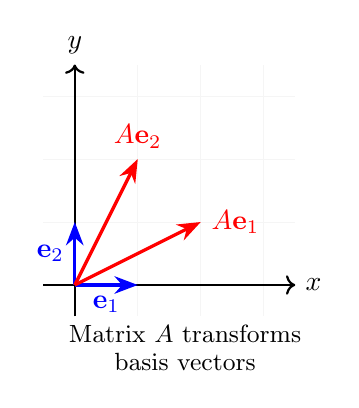
\begin{tikzpicture}[scale=0.8]
    % Grid
    \draw[lightgray, very thin] (-0.5,-0.5) grid (3.5,3.5);
    \draw[->,thick] (-0.5,0) -- (3.5,0) node[right] {$x$};
    \draw[->,thick] (0,-0.5) -- (0,3.5) node[above] {$y$};

    % Original vectors
    \draw[-{Stealth},blue,very thick] (0,0) -- (1,0) node[midway,below] {$\mathbf{e}_1$};
    \draw[-{Stealth},blue,very thick] (0,0) -- (0,1) node[midway,left] {$\mathbf{e}_2$};

    % Transformed vectors
    \draw[-{Stealth},red,very thick] (0,0) -- (2,1) node[right] {$A\mathbf{e}_1$};
    \draw[-{Stealth},red,very thick] (0,0) -- (1,2) node[above] {$A\mathbf{e}_2$};

    \node[align=center] at (1.75,-1) {\small Matrix $A$ transforms\\[-2pt]\small basis vectors};
\end{tikzpicture}
\end{center}

% ML Applications
\begin{tcolorbox}[appbox, title={\faRobot\ ML Applications}]
\begin{itemize}
    \item \textbf{Word Embeddings}: Words as vectors; similarity = dot product
    \item \textbf{Neural Networks}: Every layer is matrix multiplication + nonlinearity
    \item \textbf{PCA}: Eigendecomposition for dimensionality reduction
    \item \textbf{Recommender Systems}: Matrix factorization (SVD)
\end{itemize}
\end{tcolorbox}

% Common Pitfalls
\begin{tcolorbox}[warningbox, title={\faExclamationTriangle\ Common Pitfalls}]
\begin{itemize}
    \item Matrix multiplication is \textbf{not commutative}: $AB \neq BA$
    \item Confusing \textbf{row vectors} vs \textbf{column vectors}
    \item Forgetting that $A^{-1}$ only exists if $\det(A) \neq 0$
    \item SVD: $\Sigma$ is diagonal, $U$ and $V$ are orthogonal
\end{itemize}
\end{tcolorbox}

\end{multicols}

\vspace{5pt}
\hrule
\vspace{5pt}

% Footer
\begin{center}
\faGithub\ \textbf{Notebook}: \url{https://github.com/vijaygwu/math-powers-ai/blob/main/notebooks/ch01_linear_algebra.ipynb}
\end{center}

\end{document}
